\chapter{Design}
This chapter documents the major design decisions in the process of building a tool that supports the hinting tool concept from \ref{chap:conceptual_design}. It focuses on building models that enable translations from the use case representations to tests -- focusing on broad test coverage.

\section{Meta model}
This section discusses an evolved and simplified version of the meta model introduced in chapter \ref{chap:conceptual_design}, and covers the changes that happened when the model transitioned from concept to design.\\\\
A central concept that was removed, is the actor actions. While they provided additional information about what actors were capable of, they added little or no value to tests. The predicates that signified the pre- and postcondition have been turned into simple use blocks, which effectively means that the mapper needs to explicitly break the execution within the conditional steps, in the case of an unmet condition.
\begin{figure}[!htbp]
  \centering
  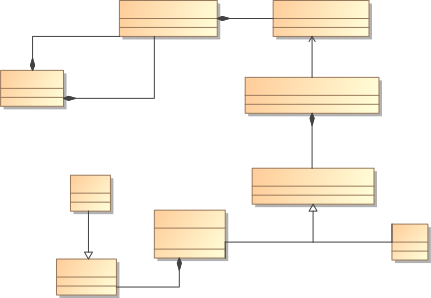
\includegraphics[scale=0.9]{img/3rd_iteration_meta_model}
  \caption{Meta model of the third concept}
  \label{fig:3rd_iteration_meta_model}
\end{figure}
When performing a translation, every use case step will be broken down into a set of decomposed steps. A decomposed step is an \emph{ordered} list of either a definition or just a text.
%TODO maybe an object diagram showing the concept.

\section{Translating a use case}
%IMPORTANT
Translation of a use case is merely unfolding its paths and generating the test function calls. The signatures of the functions are automatically inferred by the types added in the hinting phase.

We treat the use case scenario with extensions as a directed graph -- potentially containing cycles. Every node of the graph represents a use case step and every edge the invocation of the next step.

\subsection{Determining paths}
%This is, most definitely a non-trivial problem.
%It is a directed cyclic graph (acyclic if no extensions loop).
In order to find all possible paths in a use case, a depth-first search or the more efficient one based upon Warshall's Theorem\cite{rubin1978enumerating} may be used to enumerate them. Once a list of paths is retrieved, it is possible to convert every path, which is essentially a list of active actions either performed by, or affecting, the primary actor.\\\\
This list will be translated into a test by converting it into code snibblet, and join them together in a code block that becomes the body of a test function.
\subsection{Use case paths}
\label{ssec:use-case-paths}
\begin{figure}[!htbp]
\centering
\begin{tikzpicture}[->,>=stealth',shorten >=0.8pt,auto,node distance=1.8cm,
thick,
visited node/.style={circle,fill=blue!20,draw,font=\sffamily\bfseries},
extension1 node/.style={circle,fill=orange!20,draw,font=\sffamily\bfseries},
chosen node/.style={circle,fill=green!20,draw,font=\sffamily\bfseries}]

%Scenario
\node[chosen node] (s1) {$s_1$};
\node[chosen node] (s2) [below of=s1] {$s_2$};
\node[chosen node] (s3) [below of=s2] {$s_3$};
\node[chosen node] (s4) [below of=s3] {$s_4$};
\node[chosen node] (s5) [below of=s4] {$s_5$};

%Extension 1
\node[visited node] (e1_1) [left of=s2] {$e_{1.1}$};

%Extension 2
\node[extension1 node] (e2_1) [right of=s4] {$e_{2.1}$};


%Paths
\path[every node/.style={font=\sffamily\small}]
(s1)   edge node [] {} (s2)	
(s2)   edge node [] {} (s3)
       edge node [] {} (e1_1)
(s3)   edge node [] {} (s4)
(s4)   edge node [] {} (s5)
       edge node [] {} (e2_1)
(e1_1) edge[bend right] node [] {} (s3)
(e2_1) edge[bend right] node [] {} (s2)
;
\end{tikzpicture}
\caption{Graph depicting different paths through a use case}
\label{fig:application graphs}
\end{figure}
Back edges can occur, and this raised the bar, as it introduces loops. The loop detection is quite simple if we disallow nested extensions. In that case, the loop detection can be performed solely by detecting that the return point of the extension is not before the entry point in the main scenario. Loops make it impossible to achieve 100\% test coverage, as we must decide on upper bounds for the loops that are, potentially, infinite.

Extensions may be covered in two ways. Just test the single extension with respect to the main scenario (the ``happy path''), or with respect to the other extensions as well.



%The basic rules for path collection is;
\section{Mapping the test to the domain}
%TODO mention errors, how to emulate errors. We need to have a use case that describes the exact circumstances under which the error arises.
In order to write up functions that implement the generated function block stubs in actual system behavior, a programming model is presented in this section.

\section{Use case concepts}
This section discussed the individual components of a use case in the perspective of converting it into an executable test. But before venturing forth, we need to outline the concept of \emph{system state}, as it is referred in the following sections.

\subsection{Mapping branches}
Use cases may branch out and go to alternatives actions. These branches are associated with errors, and may be difficult to emulate. One possibility is to use an assumption mapping here, and treat the event or decision as having occurred. For active decisions taken by the primary actor, for example an action taken to better serve a customer request, it is easy to assume. Injecting errors in a running system is something else entirely... %TODO Finish.

\subsection{System state}
%TODO relate this to preconditions.
Well-formed use cases  know are completely self-contained\cite{larman2005} in the way that every action and alternative, for a given actor, may be put into a single (large) use case. Use cases may also specify some expectations to the system state. This is what is defined as preconditions. If we, however, maintain a system state analogy, we may model use case executions as a set of mutation functions that affect the global system state.\\\\
A simple example; a actor \emph{accountant} has a use case \emph{accountant creates invoice}. This use case requires that the \emph{accountant} actor has previously been created. The creation could be provided by the \emph{admin} actor's \emph{admin creates accountant} use case.
\begin{figure}[h]
\includegraphics[scale=0.75]{\imgdir system-state-machine-relations}
\centering
\caption{State machine of perceived system state}
\label{fig:system-state-machine-relations}
\end{figure}
In summary, the \emph{accountant creates invoice} effectively has a precondition that is provided by \emph{admin creates accountant} to make the global state match what is expected to execute the \emph{accountant creates invoice}. The concept is illustrated in figure \ref{fig:system-state-machine-relations} where \emph{Use Case 1} is a prerequisite to \emph{Use Case 2}, but \emph{Use Case 3} has no prerequisites. In order to reach completion (termination) and coverage of \emph{Use Case 2}, \emph{Use Case 1} has to be executed.\\
Each use case state (an example is \textbf{UC1} in figure \ref{fig:system-state-machine-relations}) is a super-state that contains the state space of every alternative scenario. Basically, every node, of every path extracted from the graphs described in section \ref{ssec:use-case-paths} is also a state, and every edge; the mutation function.\\\\
This model is useful to consider when programming the test support tools, and may even be supported by a concept, such as the event stack validation described in appendix \ref{appendix:event-stack-validation}, where the states and transitions are logged, and replayed through a set of state machines. But, for the majority of implementations, it should be considered a programming model. Using this model, developers may also chose to build their precondition mappings as other use cases.


\section{Test case state}
\label{sec:test_case_state}

A test consists of three basic steps; setup, run and teardown. Setup and teardown is different from pre- and postcondition in that they are unrelated to the test itself, they merely make sure that objects are initialized with right values and, in general, are in the state that the test expects.

There needs to be an executable domain model programmed, not necessarily complete, but the concepts covered in the use cases should at least be there. So for the use case ``Send message to contact'' (see appendix \ref{appendix:use-cases}). We need at least a class representing the actor ``Receptionist'', and a class representing a message. The actions performed by the actor could then either be class methods, or simply functions taking the primary actor (or more exact; classes of the actor), as an argument.

\section{Executable use case}
This section discusses a programming model and possible system designs that supports executing use cases. The basic concept is that every test is regarded as a function.
%Put this in; how many functions are in a test?
At this point, we have also identified some constraints for use cases in regards to test generation. They are left here as a note
\begin{description}
  \item[Entries:] Every entry in a use case scenario is modeled as a synchronous self-contained action.
  \item[Termination:] A use case scenario should always terminate.
\end{description}
\subsection{Environment}
\label{sec:test-environment}
\textbf{!Unfinished!}\\
Executing the use case can be considered a long function call-chain. Each new function call passes along the current global state onto the next procedure. This method of passing along the state is a common pattern is interpreters and compilers, where the global state is referred to as "the environment". In our test-case compiler we adopt this approach. One of the large benefits is to have the ability to have an exit procedure that performs state clean upon exit of every use case. These procedures should run regardless of exceptions raised within the call-chain, but respond to them. This behavior is identical to the functionality seen in "teardown" functions in test framework for programming languages.\\\\
The environment should contain the current state within the scope of test currently running. By state is meant any objects created or modified during the test.
The expression of a use case that consists of $n$ statements then becomes: 
\begin{equation}
Postcondition \rightarrow S_n \rightarrow S_{n-1} \rightarrow \dotsb \rightarrow S_2 \rightarrow S_1 \rightarrow Precondition \rightarrow env
\end{equation}
The expression function is applied to the statement, then the result is applied to the matcher which then returns a success or failure value depending on the outcome of the evaluation.
%TODO This is (maybe) conceptually a monad.
%\texttt{matcher expression} ($s$)

%\begin{algorithmic}
%\If {$i\geq maxval$}
%    \State $i\gets 0$
%\Else
%    \If {$i+k\leq maxval$}
%        \State $i\gets i+k$
%    \EndIf
%\EndIf
%\end{algorithmic}
%TODO the requirements to the state is inferred by the used concepts.

\subsection{Mapping entries}
Any use case statement may be mapped to an assumption, an error or an assumption.


\subsection{Detecting logic errors in use cases}

\begin{description}
  \item[Skipping actions may be prohibited:] Should it be possible to jump ahead in the use case?
  \item[Primary actor must participate:] The primary actor is important, as this is the stakeholder that defines the perspective and scope of the test. The primary is the person that starts the use case via an active action, or receives a start signal from another actor -- the system for instance. The primary actor must also be part of the main scenario, and an analysis error should occur if this is not the case.

\end{description}


%TODO there are problems with duplicate words; table table.

%TODO Integrate and finalize notes below.

% A use case returns a outputstate which is composed by an outputlog (log messages). A list of assumptions or an error. An error is for when an expectation failed, or a system error occured. Assumptions are for use case entries that are mapped to assumption statements.



%\section{Test framework}
% You need to write a test framework containing object pools, factory classes aso.
%\subsection{Exploiting injected semantics}
%How may we benefit from additional semantics? We can identify rubbish postconditions, such as predicates that involve objects that are either not modified in the statements, or simply never referenced.

%\section{Evaluating a use case}
%A use case can be modeled as a function taking in a starting environment and returning a boolean value, so $U \rightarrow env \rightarrow bool$


%Test case; when does it end? in our case, the message-sending archtecture is defined to be a work-queue where the dispatcher is decoupled from the message sending, which is merely an enqueuer. If the postcondition for our test case had been; "Message is received by contact", then the test-macro function becomes increasingly large.
%Test cases may further introduce dependencies, such as messageStore

%On the interface side, we decided that 2xx series HTTP codes where mapped to normal responses, and 4xx and 5xx to execeptions. 1xx and 3xx series are unused in our stak, and thus, unmapped. But it provides us with a good tool for -- on the client -- to explicitly state which replies should go where, and how they should be handled.


\subsection{Running the analysis}
Having a set of definitions, we can detect actors and concepts from textually analysing the text of every UseCaseEntry object. The analysis is quite simple, and merely looks for occurrences of the definition by comparing strings.



\subsection{Capabilites of an actor}
If we were to add additional domain knowledge to the use cases, then we would also be able to extract capabilities easily.
%yada yada, use case example: actor does something to some other thing
% it means the the actor can do something to some other thing.

\subsection{Providing initial information}
%How to add receptions, users and other stuff?
%Could this be done with a use case as well?

\subsection{Configuration environment}
How do we define which objects are currently in the test harness? In our implementation, we have made a configuration file that, potentially could be auto-generated from a description of which domain types the objects have, what their internal data is, and when they need to be present.

